% CS615A Aspects of System Administration
% Author: Jan Schaumann <jschauma@netmeister.org>
% $Id: slides.tex,v 1.12 2006/02/12 23:15:03 jschauma Exp $

\special{! TeXDict begin /landplus90{true}store end }

\documentclass[xga]{xdvislides}
\usepackage[landscape]{geometry}
\usepackage{graphics}
\usepackage{graphicx}
\usepackage{colordvi}
\usepackage{tabularx}
\usepackage{multirow}

\newcommand{\smallish}{\fontsize{16}{16}\selectfont}

\begin{document}
\setfontphv

%%% Headers and footers
\lhead{\slidetitle}                               % default:\lhead{\slidetitle}
\chead{CS615 - Aspects of System Administration}% default:\chead{\relax}
\rhead{Slide \thepage}                       % default:\rhead{\sectiontitle}
\lfoot{\Gray{Multiuser Fundamentals}}% default:\lfoot{\slideauthor}
\cfoot{\relax}                               % default:\cfoot{\relax}
\rfoot{\Gray{\today}}

\vspace*{\fill}
\begin{center}
	\Hugesize
		CS615 - Aspects of System Administration\\ [1em]
		Multiuser Fundamentals\\ [1em]
	\hspace*{5mm}\blueline\\ [1em]
	\Normalsize
		Department of Computer Science\\
		Stevens Institute of Technology\\
		Jan Schaumann\\
		\verb+jschauma@stevens.edu+\\
		\verb+https://www.cs.stevens.edu/~jschauma/615/+
\end{center}
\vspace*{\fill}

\subsection{Multiuser}

UNIX was designed from the beginning (1970s) as a portable, multi-tasking,
{\em multi-user} system. \\

Windows gained this functionality with WindowsNT in 1993. \\

Mac OS followed in 2001 with OS X.

\subsection{Implications of a Multi-User System}
\vspace*{\fill}
\begin{center}
	\includegraphics[scale=0.8]{pics/teamwork.eps}
\end{center}
\vspace*{\fill}

\subsection{Implications of a Multi-User System}
\vspace*{\fill}
\begin{center}
	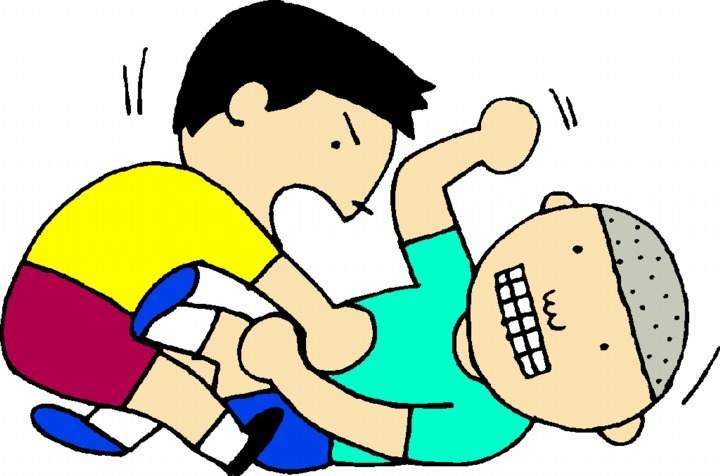
\includegraphics[scale=0.7]{pics/kids_fighting.eps}
\end{center}
\vspace*{\fill}

\subsection{Consider Scalability}
Things to consider:
\\

\begin{center}
	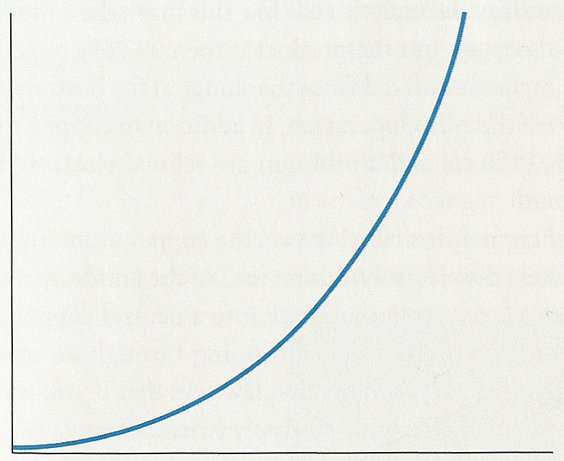
\includegraphics[scale=2.8]{pics/exponential_growth.eps}
\end{center}


\subsection{Granting Privileges requires Trust}
\begin{itemize}
	\item different environments have different trust models
	\item human interactions in small groups strengthen trust
	\item larger groups are divided into smaller, close-nit groups
	\item the more groups you have, the weaker their trust bonds are
\end{itemize}

\subsection{Granting Privileges requires Trust}
\begin{itemize}
	\item different environments have different trust models
	\item human interactions in small groups strengthen trust
	\item larger groups are divided into smaller, close-nit groups
	\item the more groups you have, the weaker their trust bonds are
\end{itemize}
\vspace{.5in}

\begin{center}
	\Huge
	{\bf Trust does not scale.}
	\Normalsize
\end{center}

\subsection{Granting Privileges requires Trust}
\Huge
We are considering {\em computer-human systems}. \\

\vspace{.5in}
For humans, trust, but (be able to) verify. \\

\vspace{.5in}
For computers, apply the {\em Least Privilege} principle. \\
\Normalsize

\subsection{Implications of a Multi-User System}
\begin{itemize}
	\item users may want to keep files private
\end{itemize}

\subsection{Implications of a Multi-User System}
\begin{itemize}
	\item users may want to keep files private
	\item users may want to share files
\end{itemize}

\subsection{Implications of a Multi-User System}
\begin{itemize}
	\item users may want to keep files private
	\item users may want to share files
	\item users may (try to gain) access to files they shouldn't have access to
\end{itemize}

\subsection{Implications of a Multi-User System}
\begin{itemize}
	\item users may want to keep files private
	\item users may want to share files
	\item users may (try to gain) access to files they shouldn't have access to
	\item users may (want to) do things that affect other users
\end{itemize}

\subsection{Implications of a Multi-User System}
\begin{itemize}
	\item users may want to keep files private
	\item users may want to share files
	\item users may (try to gain) access to files they shouldn't have access to
	\item users may (want to) do things that affect other users
	\item different users may require different privileges
\end{itemize}

\subsection{Users and User-IDs}
\begin{center}
	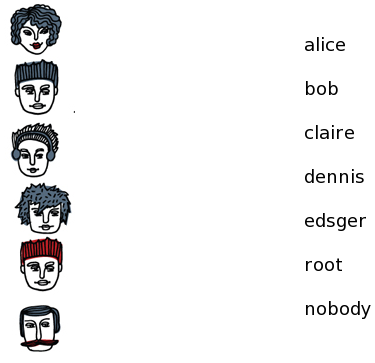
\includegraphics[scale=0.9]{pics/user-sets0.eps} \\
	Bijective?
\end{center}

\subsection{Users and User-IDs}
\begin{center}
	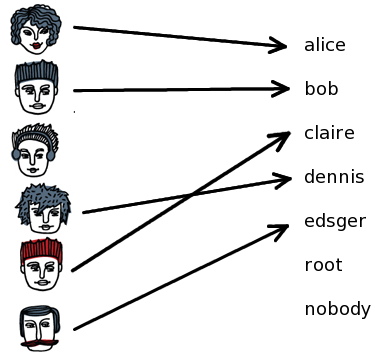
\includegraphics[scale=0.9]{pics/user-sets1.eps} \\
	{\em Not} surjective!
\end{center}

\subsection{Users and User-IDs}
\begin{center}
	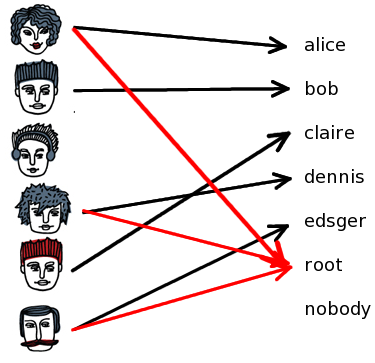
\includegraphics[scale=0.9]{pics/user-sets2.eps} \\
	{\em Not} injective, either!
\end{center}

\subsection{Users and User-IDs}

\begin{center}
	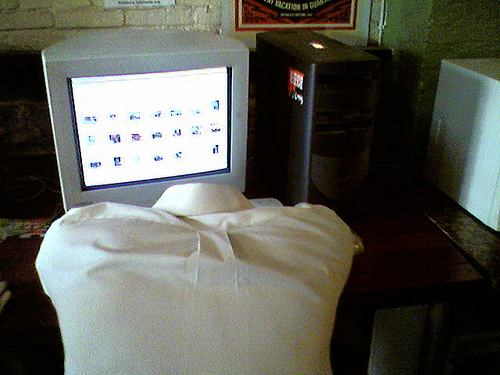
\includegraphics[scale=0.8]{pics/headless.eps} \\
	{\tt nobody}
\end{center}

%\subsection{Implications of a Multi-User System}
%\vspace*{\fill}
%\begin{center}
%	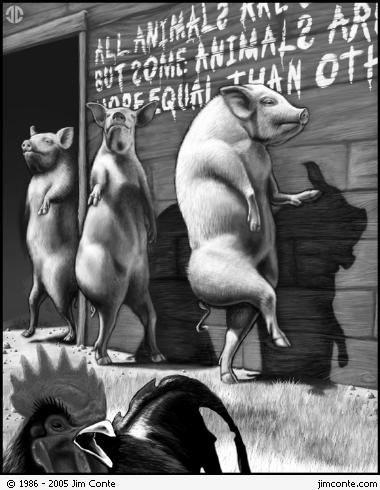
\includegraphics[scale=0.9]{pics/animal_farm.eps}
%\end{center}
%\vspace*{\fill}
%
\subsection{Authentication}

\begin{itemize}
	\item proof of identity, not proof of {\em authorization}
\end{itemize}

\subsection{Authentication}

\begin{itemize}
	\item proof of identity, not proof of {\em authorization}
	\item something you know, something you have, something you are
\end{itemize}

\subsection{Authentication}

\begin{itemize}
	\item proof of identity, not proof of {\em authorization}
	\item something you know, something you have, something you are
	\item multi-factor authentication combines these to help protect against different threats
\end{itemize}

\subsection{Authentication}

\begin{itemize}
	\item proof of identity, not proof of {\em authorization}
	\item something you know, something you have, something you are
	\item multi-factor authentication combines these to help protect against different threats
	\item mutual authentication may be a requirement
\end{itemize}

\subsection{Authentication}
Common examples:

\begin{verbatim}
NetBSD/amd64 (SERVER) (console)

login: jschauma
password: *********************************
NetBSD 7.0.2 (SERVER) #2: Tue Jan 24 02:33:13 EST 2017

Welcome to NetBSD!
hostname$ 
\end{verbatim}

\subsection{Authentication}
Common examples:

\begin{verbatim}
$ ssh-keygen -l -f /dev/stdin <<<$(aws ec2 get-console-output \
        i-0990f1eb069c853c4 | grep ^ecdsa)
256 19:af:35:01:0b:2a:ee:3d:30:0f:69:11:cc:55:7c:20 (ECDSA)
$ ssh -i ~/.ssh/myawskey ec2-54-227-16-184.compute-1.amazonaws.com
The authenticity of host 'ec2-54-227-16-184.compute-1.amazonaws.com
(54.227.16.184)' can't be established.
ECDSA key fingerprint is 19:af:35:01:0b:2a:ee:3d:30:0f:69:11:cc:55:7c:20.
Are you sure you want to continue connecting (yes/no)?  yes
NetBSD 7.0.2 (SERVER) #2: Tue Jan 24 02:33:13 EST 2017

Welcome to NetBSD!
hostname$ 
\end{verbatim}

\subsection{Authentication}
Common examples:

\begin{verbatim}
$ kinit
Password for jschauma@DOMAIN: ********************************
$ klist
Ticket cache: /tmp/krb5cc_ttypa
     Default principal: jschauma@DOMAIN
     
     Valid starting     Expires            Service principal
     02/13/17 13:50:21  02/13/17 21:50:20  krbtgt/KDC@DOMAIN
$ ssh somehost
somehost$ 
\end{verbatim}

\subsection{Authentication}
Common examples:

\smallish
\begin{verbatim}
localhost$ ssh sshca
YubiKey for `jschauma': ********************************
Password: ********************************
localhost$ ssh-add -l
2048 SHA256:TzwuHGc5BKBe+VJSnGoVyh92J8XKBUkaL7MGQn8ML0Y (RSA)
2048 SHA256:TzwuHGc5BKBe+VJSnGoVyh92J8XKBUkaL7MGQn8ML0Y (RSA-CERT)
localhost$ ssh somehost
Duo two-factor login for jschauma

Enter a passcode or select one of the following options:

 1. Duo Push to XXX-XXX-0712
 2. Phone call to XXX-XXX-0712
 3. SMS passcodes to XXX-XXX-0712

Passcode or option (1-3): 1
Success. Logging you in...
Last login: Thu Jan 26 17:39:30 2017 from 10.1.2.3

somehost$ 
\end{verbatim}
\Normalsize

\subsection{Authentication}
Common examples:
\vfill
\begin{center}
	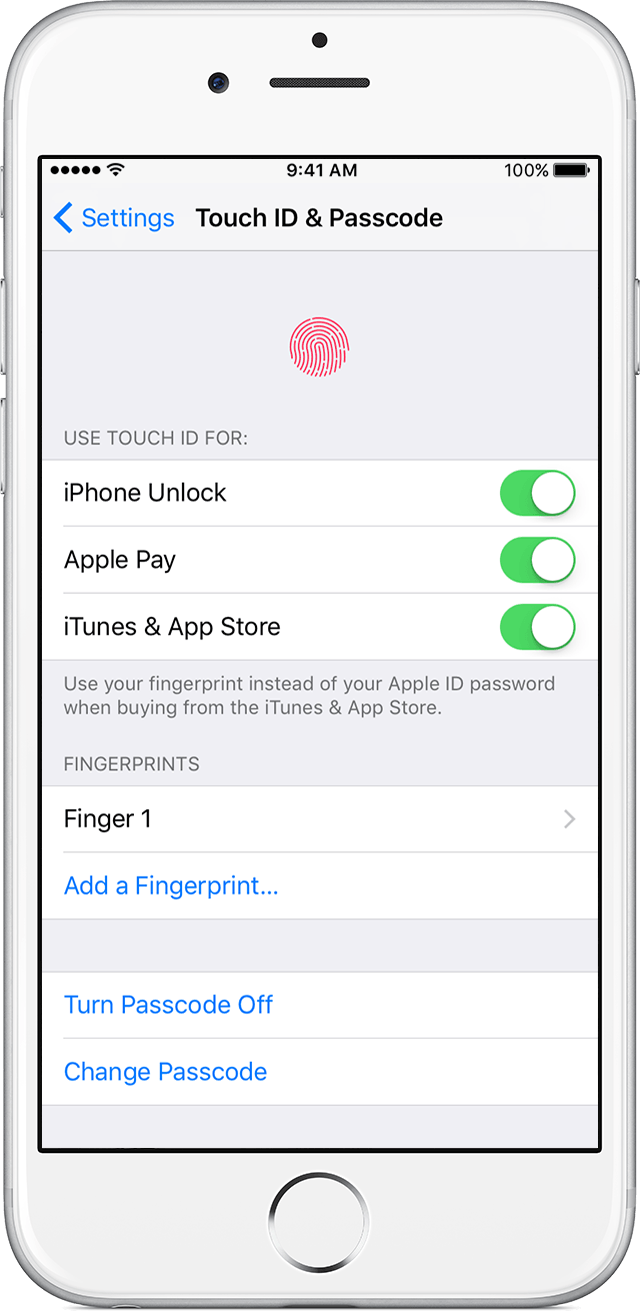
\includegraphics[scale=0.25]{pics/iphone.eps}
\end{center}
\vfill

\subsection{Authentication}
Common examples:
\begin{itemize}
	\item passwords, PINs
	\item ssh keys, PGP keys, X.509 certificates
	\item security tokens: OTPs in hardware or software, RFIDs
	\item physical biometrics: fingerprint, retina scan, facial recognition
	\item behavioral biometrics: speech pattern, gait, keystroke dynamics...
\end{itemize}
\vspace{.5in}

Mix and match the above to yield multi-factor
authentication:
\begin{itemize}
	\item password + PIN via e.g. SMS
	\item ssh key + TOTP from e.g. mobile device
	\item fingerprint + security token
	\item ...
\end{itemize}


\subsection{UNIX Fundamentals: User Accounts and File Permissions}
Every account
\begin{itemize}
	\item has a {\em unique} ID
	\item belongs to at least one group
	\item may or may not be password protected
	\item may or may not have a valid login program
	\item may or may not be allowed to escalate privileges
\end{itemize}

\subsection{UNIX Fundamentals: User Accounts and File Permissions}
Every account
\begin{itemize}
	\item has a {\em unique} ID
	\item belongs to at least one group
	\item may or may not be password protected
	\item may or may not have a valid login program
	\item may or may not be allowed to escalate privileges
\end{itemize}
\addvspace{.5in}
Every file
\begin{itemize}
	\item is associated with a {\em uid} and a {\em gid}
	\item has a number of protection bits
\end{itemize}

\subsection{UNIX Fundamentals: User Accounts and File Permissions}
\vfill
\begin{center}
	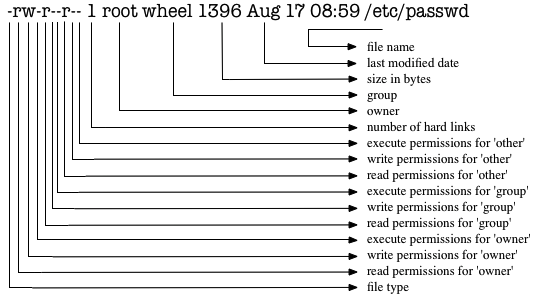
\includegraphics[scale=0.9]{pics/ls-l.eps}
\end{center}
\vfill

\subsection{Raising privileges}
Some tasks require special privileges:
\begin{itemize}
	\item binding a port $< 1024$ (e.g. 22, 25, 80, 443)
	\item operating on raw sockets (e.g. {\tt ping(1)}, {\tt traceroute(8)})
	\item changing local passwords
	\item accessing files/directories without explicit permissions
	\item just about anything involving file systems
	\item ...
\end{itemize}

\subsection{Raising privileges}
Options:

\begin{verbatim}
somehost$ exit
$ ssh root@somehost
# 
\end{verbatim}

\subsection{Raising privileges}
Options:

\begin{verbatim}
$ su user2 -c 'some command'
Password:
$ su - root
Password:
# 
\end{verbatim}

\subsection{Raising privileges}
Options:

\begin{verbatim}
somehost$ sudo bash
jschauma is not allowed to run sudo on somehost.  This incident will be reported.
\end{verbatim}

\subsection{Raising privileges}
Options:

\begin{verbatim}
jschauma@somehost$ ls dir
ls: cannot open directory dir: Permission denied
jschauma@somehost$ sudo bash
Sorry, user jschauma is not allowed to execute '/bin/bash' as root on somehost.
jschauma@somehost$ sudo ls dir
Sorry, user jschauma is not allowed to execute '/bin/ls' as root on somehost.
jschauma@somehost$ sudo -u otheruser ls dir
Password: ********************************
file1   file2
jschauma@somehost$ 
\end{verbatim}

\subsection{Unix Groups}
\begin{itemize}
	\item enables {\em arbitrary} collections of users to share resources
	\item information stored in \verb+/etc/group+, format is: \\
		\verb+name:*:GID:user1,user2,...+
	\item most Unix systems impose a limit of 16 or 32 group memberships per
		user
	\item most Unix systems have a common default group for new users (some
		Linux versions deviate)
	\item some Unix systems have/had group shadow files
\end{itemize}

\subsection{Group Access}
At any but the smallest environments, we find:
\begin{itemize}
	\item a central user database
	\item users divided into different access groups
	\item access to systems is granted primarily by such group membership
	\item privileges on a system are also granted by such group membership
\end{itemize}
\vspace{.5in}
The privileges granted in this manner are commonly
broken down and controlled via {\em role-based access
control} (RBAC).

\subsection{Group Access}
\begin{center}
	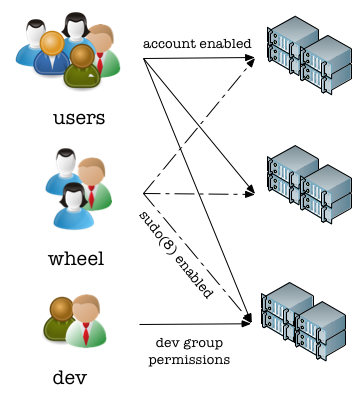
\includegraphics[scale=0.8]{pics/groups-machines.eps}
\end{center}

\subsection{Multiuser Truths}
\begin{itemize}
	\item {\em All users are equal.}
	\item {\em Some users are more equal than others.}
	\item {\em The principle of least privilege applies to all.}
	\item {\em Humans require trust.}
	\item {\em Trust does not scale.}
	\item {\em You will always face trade-offs.}
\end{itemize}


\subsection{Adding and Removing Accounts}

\vfill
In-class exercise: \\
\verb+https://www.cs.stevens.edu/~jschauma/615/useradd-exercise.html+
\vfill

%\subsection{Adding and Removing Accounts}
%\vfill
%In-class exercise: \\
%\verb+http://www.cs.stevens.edu/~jschauma/615/useradd-exercise.html+
%
%\vspace{.5in}
%Accounts management is done centrally; changes are applied to machines via a
%configuration management system and/or directory service.
%\vfill

%\subsection{Ethics}
%\begin{center}
%	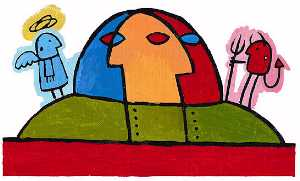
\includegraphics[scale=2.5]{pics/angel-devil.eps}
%\end{center}
%
%\subsection{You are a Super User!}
%\begin{center}
%	
\includegraphics[scale=1.0]{pics/superman.eps} \\
%	\small
%	Yes, you are!
%	\Normalsize
%\end{center}
%
%\subsection{You are a Super User!}
%\begin{center}
%	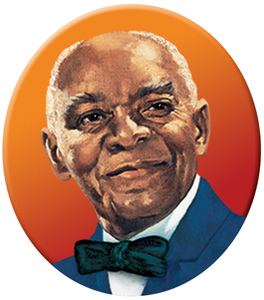
\includegraphics[scale=4.0]{pics/uncle-ben.eps} \\
%	\addvspace{.2in}
%	\Huge
%	``With great power comes great responsibility.''
%	\Normalsize
%\end{center}
%
%\subsection{sudo(8)}
%\vspace*{\fill}
%\begin{verbatim}
%We trust you have received the usual lecture from the local System
%Administrator. It usually boils down to these three things:
%#1) Respect the privacy of others.
%#2) Think before you type.
%#3) With great power comes great responsibility.
%\end{verbatim}
%\vspace*{\fill}
%
%\subsection{Ethics}
%The LISA Code of Ethics:
%\\
%
%\newcolumntype{S}{>{\centering\arraybackslash} m{.4\linewidth} }
%\begin{tabular}{ p{10cm} S }
%\begin{itemize}
%	\item Professionalism
%	\item Personal Integrity
%	\item Privacy
%	\item Laws and Policies
%	\item System Integrity
%	\item Education
%	\item Social Responsibility
%	\item Ethical Responsibility
%\end{itemize}
%& \multirow{20}{*}{
\includegraphics[scale=1.3]{pics/angel.eps}} \\
%\end{tabular}
%
%\subsection{Ethics: This stuff isn't easy!}
%\begin{center}
%	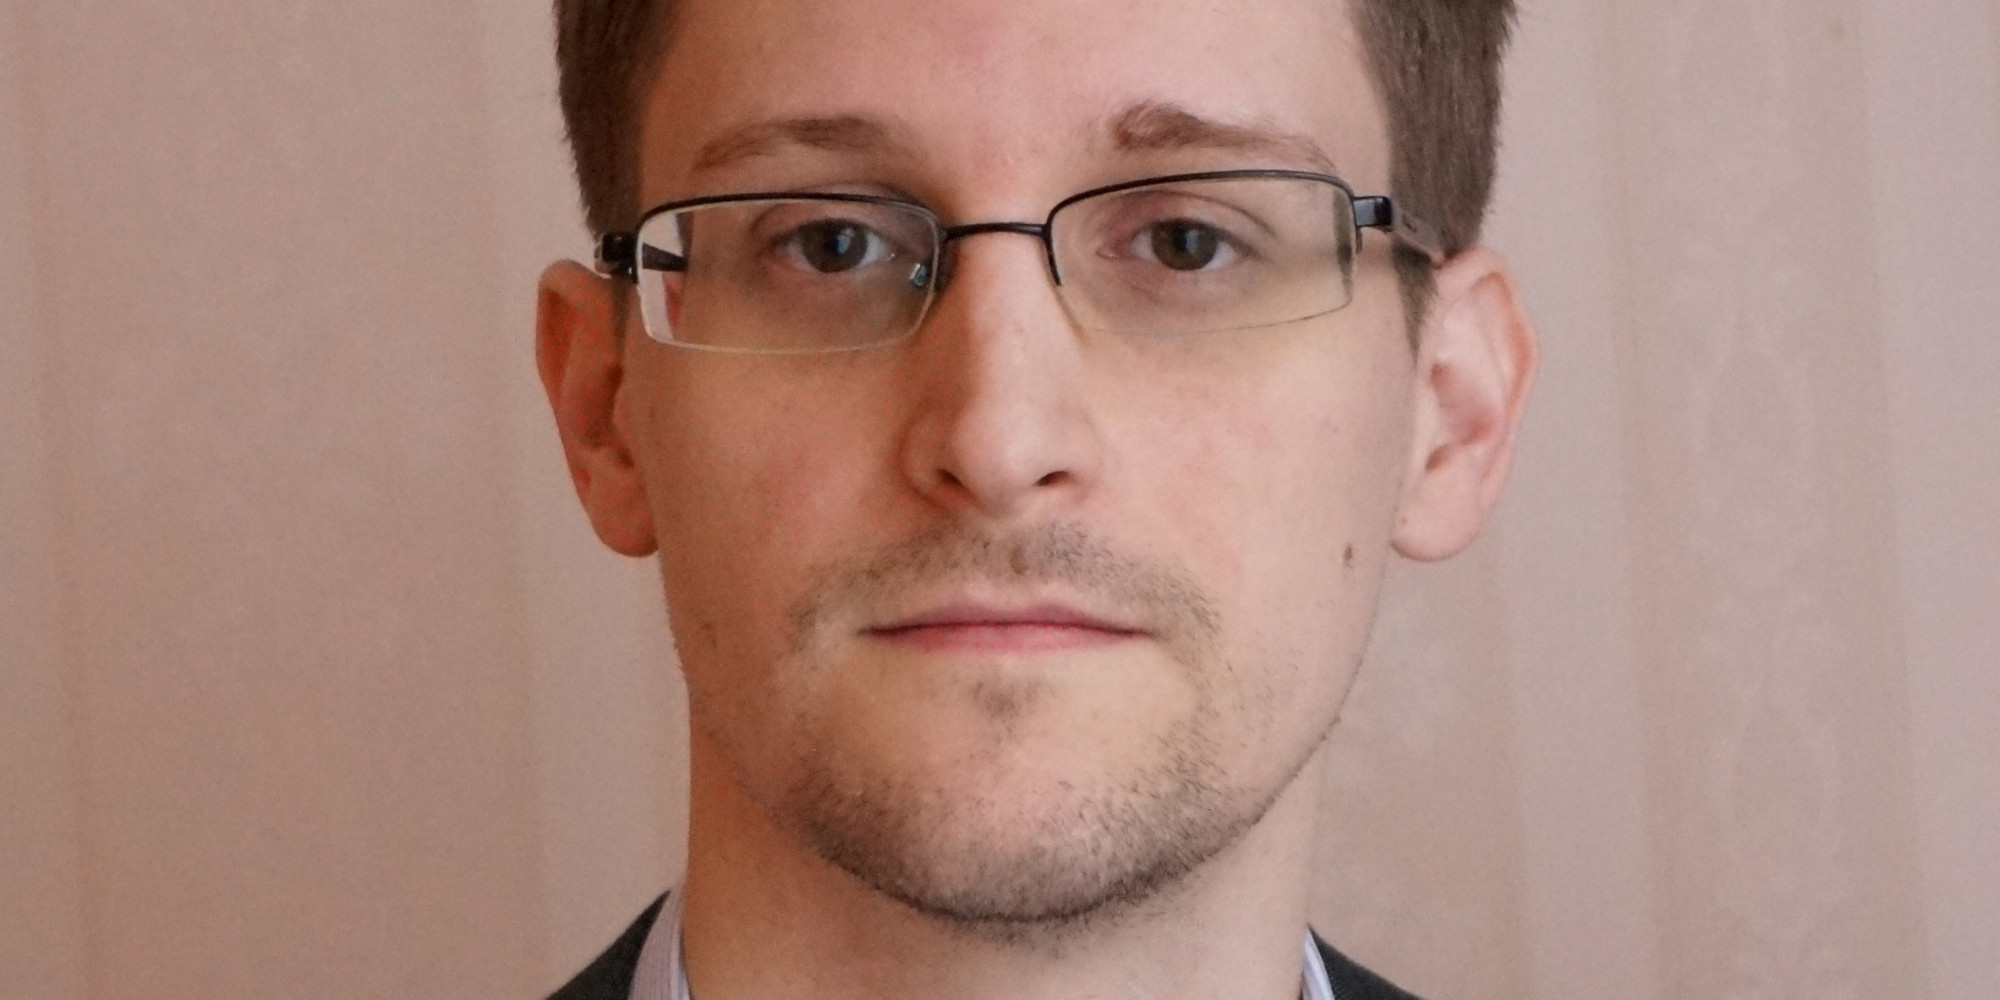
\includegraphics[scale=0.3]{pics/snowden.eps}
%\end{center}
%
%\subsection{Ethics: Professionalism}
%\vfill
%\begin{center}
%I will maintain professional conduct in the workplace and will not allow
%personal feelings or beliefs to cause me to treat people unfairly or
%unprofessionally.
%\end{center}
%\vfill
%
%\subsection{Ethics: Personal Integrity}
%\vfill
%\begin{center}
%I will be honest in my professional dealings and forthcoming about my
%competence and the impact of my mistakes. I will seek assistance from
%others when required. \\
%\vspace{.5in}
%
%I will avoid conflicts of interest and biases whenever possible. When my
%advice is sought, if I have a conflict of interest or bias, I will declare
%it if appropriate, and recuse myself if necessary.
%\end{center}
%\vfill
%
%
%\subsection{Ethics: Privacy}
%\vfill
%\begin{center}
%I will access private information on computer systems only when it is
%necessary in the course of my technical duties. I will maintain and
%protect the confidentiality of any information to which I may have access,
%regardless of the method by which I came into knowledge of it.
%\end{center}
%\vfill
%
%\subsection{Ethics: Laws and Policies}
%\vfill
%\begin{center}
%I will educate myself and others on relevant laws, regulations, and
%policies regarding the performance of my duties.
%\end{center}
%\vfill
%
%\subsection{Ethics: Communication}
%\vfill
%\begin{center}
%I will communicate with management, users, and colleagues about computer
%matters of mutual interest. I will strive to listen to and understand the
%needs of all parties.
%\end{center}
%\vfill
%
%\subsection{Ethics: System Integrity}
%\vfill
%\begin{center}
%I will strive to ensure the necessary integrity, reliability, and
%availability of the systems for which I am responsible. \\
%\vspace{.5in}
%
%I will design and maintain each system in a manner to support the
%purpose of the system to the organization.
%\end{center}
%\vfill
%
%\subsection{Ethics: Education}
%\vfill
%\begin{center}
%I will continue to update and enhance my technical knowledge and other
%work-related skills. I will share my knowledge and experience with others.
%\end{center}
%\vfill
%
%\subsection{Ethics: Responsibility to the Computing Community}
%\vfill
%\begin{center}
%I will cooperate with the larger computing community to maintain the
%integrity of network and computing resources.
%\end{center}
%\vfill
%
%\subsection{Ethics: Social Responsibility}
%\vfill
%\begin{center}
%As an informed professional, I will encourage the writing and adoption of
%relevant policies and laws consistent with these ethical principles.
%\end{center}
%\vfill
%
%\subsection{Ethics: Ethical Responsibility}
%\vfill
%\begin{center}
%I will strive to build and maintain a safe, healthy, and productive
%workplace. \\
%\vspace{.5in}
%
%I will do my best to make decisions consistent with the safety, privacy,
%and well-being of my community and the public, and to disclose promptly
%factors that might pose unexamined risks or dangers. \\
%\vspace{.5in}
%
%I will accept and offer honest criticism of technical work as appropriate
%and will credit properly the contributions of others. \\
%\vspace{.5in}
%
%I will lead by example, maintaining a high ethical standard and degree
%of professionalism in the performance of all my duties. I will support
%colleagues and co-workers in following this code of ethics.
%
%\end{center}
%\vfill
%
%\subsection{SysAdmin realities}
%\begin{itemize}
%	\item you are in a {\em privileged} position
%\end{itemize}
%
%\subsection{SysAdmin realities}
%\begin{itemize}
%	\item you are in a {\em privileged} position
%	\item you {\em are} a target
%\end{itemize}
%
%\subsection{SysAdmin realities}
%\begin{itemize}
%	\item you are in a {\em privileged} position
%	\item you {\em are} a target
%	\item you are {\em obligated} to act in your users' interest
%\end{itemize}
%
%\subsection{SysAdmin realities}
%\begin{itemize}
%	\item you are in a {\em privileged} position
%	\item you {\em are} a target
%	\item you are {\em obligated} to act in your users' interest
%	\item you {\em will} face tough choices
%\end{itemize}
%
%\subsection{SysAdmin realities}
%\begin{itemize}
%	\item you are in a {\em privileged} position
%	\item you {\em are} a target
%	\item you are {\em obligated} to act in your users' interest
%	\item you {\em will} face tough choices
%	\item there is {\em no rulebook} to help you decide
%\end{itemize}
%
%\subsection{SysAdmin realities}
%\begin{itemize}
%	\item you are in a {\em privileged} position
%	\item you {\em are} a target
%	\item you are {\em obligated} to act in your users' interest
%	\item you {\em will} face tough choices
%	\item there is {\em no rulebook} to help you decide
%	\item you {\em can} make a difference
%\end{itemize}
%
%\subsection{At the end of the day...}
%\begin{center}
%	
\includegraphics[scale=0.5]{pics/thumbsup-borat.eps}
%\end{center}

\subsection{Reading}
User Management:
\begin{itemize}
	\item {\em Frisch}: Ch 6; {\em Burgess}: Ch 5;
\end{itemize}
\vspace{.5in}
\begin{itemize}
	\item {\tt https://is.gd/wg5OsE}
	\item {\tt https://www.netmeister.org/book/06-users-and-groups.pdf}
\end{itemize}

%\vspace{.5in}
%Ethics:
%\begin{itemize}
%	\item \verb+https://www.usenix.org/lisa/system-administrators-code-ethics+
%	\item \verb+http://www.acm.org/about/code-of-ethics+
%	\item \verb+https://www.netmeister.org/blog/primum-non-nocere.html+
%\end{itemize}
%
%\subsection{Professional Organizations}
%\begin{itemize}
%	\item \verb+https://www.usenix.org/+ and \verb+https://www.usenix.org/lisa+
%	\item \verb+http://www.lopsa.org/+
%	\item \verb+http://www.acm.org/+
%	\item \verb+https://www.internetsociety.org/+
%	\item \verb+https://www.nanog.org/+
%\end{itemize}
%
\end{document}
